\documentclass[handout]{beamer}

\usepackage{fontspec} 
\useoutertheme{lsp}

\usepackage{lsptitle}
\usepackage{booktabs}
\def\two@digits#1{\ifnum#1<10 0\fi\number#1}
\def\mytoday{\two@digits{\number\day}.\two@digits{\number\month}.\number\year}


\usepackage{xspace,multicol}
\newcommand{\latex}{\LaTeX\xspace}
\usepackage{tikz}


\newcounter{lastpagemainpart}
\footnotesep0pt
\renewcommand{\footnoterule}{}
\usefootnotetemplate{
  \noindent
  \insertfootnotemark\insertfootnotetext}

\let\beamerfn=\footnote
\renewcommand{\footnote}[1]{\%
\let\oldfnsize=\footnotesize\%
\let\footnotesize=\tiny\%
\beamerfn<\thebeamerpauses->{#1}\%
\let\footnotesize=\oldfnsize}


\date{\today}

\usepackage{eurosym}  
 
\renewcommand{\centerline}[1]{\hfill#1\hfill\hfill\mbox{}}


\title{\mbox{Community proofreading as a tool}\\
\mbox{for community engagement}\\
\small A quantitative analysis}
\institute{FU Berlin}
\author[LangSci]{Sebastian Nordhoff}



\begin{document}
\lspbeamertitle

\section{Open Access $\to$ Open Publishing}

\frame{
\frametitle{Open Publishing}
%   \includegraphics[height=.6\textheight]{./path/to/graphicsfile}
  \begin{itemize}
    \item Open Access is mainly concerned with reading 
    \item Open Publishing is concerned with making all aspects of publishing open 
    \begin{itemize}
      \item Open source platforms 
      \item Open bookkeeping 
      \item Open peer review
      \item Community proofreading
    \end{itemize}    
  \end{itemize}
}

\section{Community}
\frame{
\frametitle{Bibliodiversity}
%   \includegraphics[height=.6\textheight]{./path/to/graphicsfile}
  \begin{itemize}
    \item one research can adopt different roles 
    \begin{itemize}
      \item 
author, reviewer, reader, ...
    \end{itemize}
    \item junior researchers are more often readers 
    \item senior researchers take on the other roles as well 
    \item complex ecosystem
    \item community-based publishing tries to integrate researchers at all levels
  \end{itemize}
}


\section{Community proofreading}
\frame{
\frametitle{Traditional proofreading}
%   \includegraphics[height=.6\textheight]{./path/to/graphicsfile}
  \begin{itemize}
    \item  outsourced work-for-hire
    \item for a fee
    \item one proofreader 
    \item specialist in style and guidelines 
    \item might have some training in linguistics
    \item normally no specialist knowledge of the particular subfield 
  \end{itemize}
}

\frame{
\frametitle{Community proofreading}
%   \includegraphics[height=.6\textheight]{./path/to/graphicsfile}
  \begin{itemize}
    \item crowdsourced to the community  
    \item voluntary work 
    \item many proofreaders 
    \item very often specialists in the particular subfield 
    \item intrinsic interest 
    \item less acquaintance with style and guidelines
  \end{itemize}
}

\frame{
\frametitle{Language Science Press}
%   \includegraphics[height=.6\textheight]{./path/to/graphicsfile}
  \begin{itemize}
    \item  Open Access publisher in linguistics 
    \item 100+ books since 2014 
    \item 350 community proofreaders
  \end{itemize}
}

\frame{
\frametitle{Workflow}
  \begin{itemize}
    \item proofreading queue with a new title every 2 weeks 
    \item title is announced on Monday
    \item community members can volunteer and claim a chapter
    \item chapters are assigned on Wednesday 
    \item 4 weeks time for proofreading 
    \item proofreading is done on Paperhive
  \end{itemize}
}


\section{Study}
\frame{
\frametitle{Westedt (2018)}
Westedt analysed a sample of comments on Paperhive for her BA thesis.
\medskip 

\begin{tabular}{lr}
Category & Percentage\\
\midrule 
Spelling&
7.30\\
Syntax&
7.80\\
Lexical choice&
20.73\\
Grammar&
11.55\\
Punctuation&
11.81\\
Style&
21.00\\
\textbf{Content}&
\textbf{6.56}\\
Miscellanea&
3.41\\
References&
9.71\\
\end{tabular}
}


\frame{
\frametitle{This study}
%   \includegraphics[height=.6\textheight]{./path/to/graphicsfile}
  \begin{itemize}
    \item  52 books from late 2016 to late 2018
    \item comments were harvested from Paperhive and put into a database
    \item 19\,004 pages 
    \item 43\,370 comments
  \end{itemize}
}

\section{Descriptive statistics}
\frame{
\frametitle{Book length}
  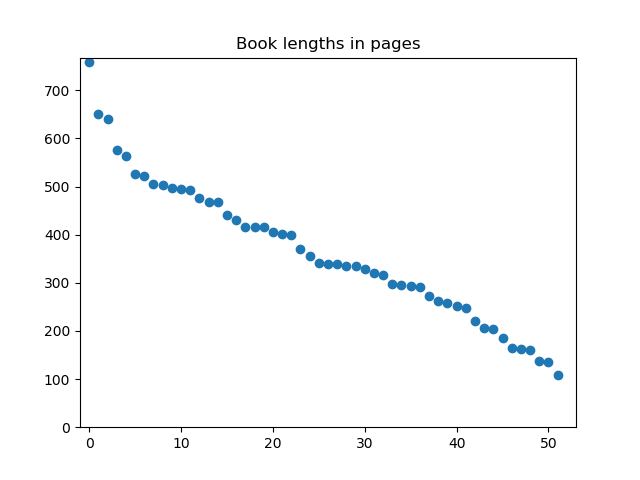
\includegraphics[height=\textheight]{booklengths_p.png}
}

\frame{
\frametitle{Comments}
  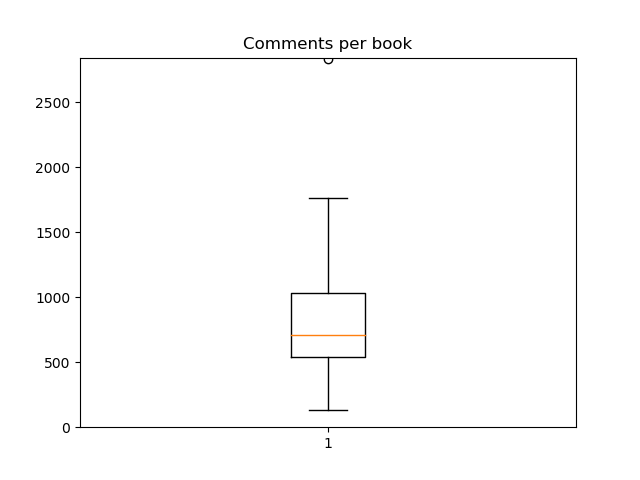
\includegraphics[height=.6\textheight]{commentsperbook.png}
  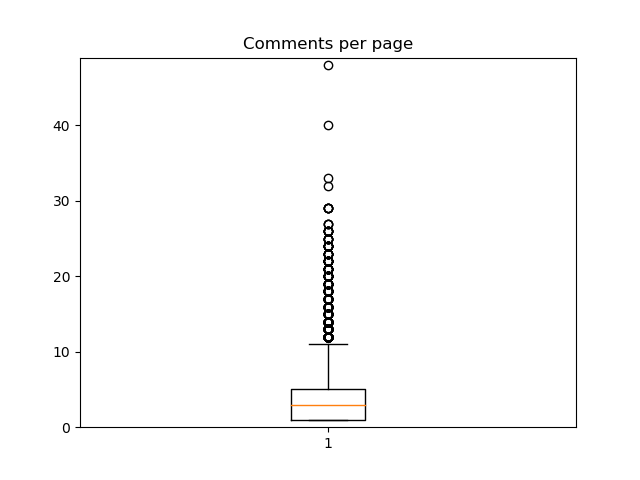
\includegraphics[height=.6\textheight]{commentsperpage.png}
The highest number of comments on one page is found in Theory and description in African Linguistics on page 122 (48 comments).
}

\frame{
\frametitle{Productivity of proofreaders}
  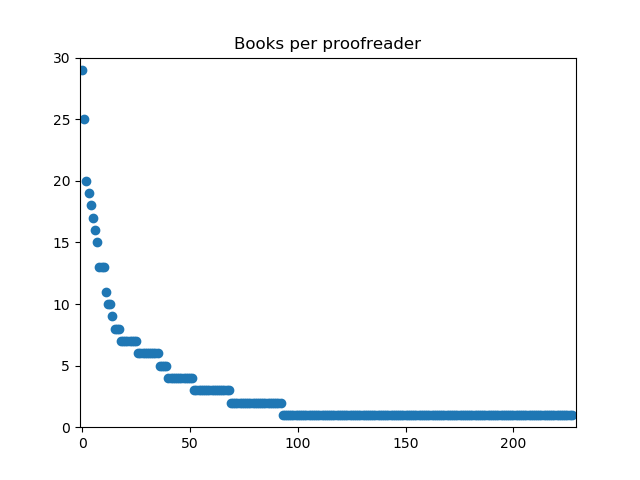
\includegraphics[height=.6\textheight]{booksperproofreader_p.png}
  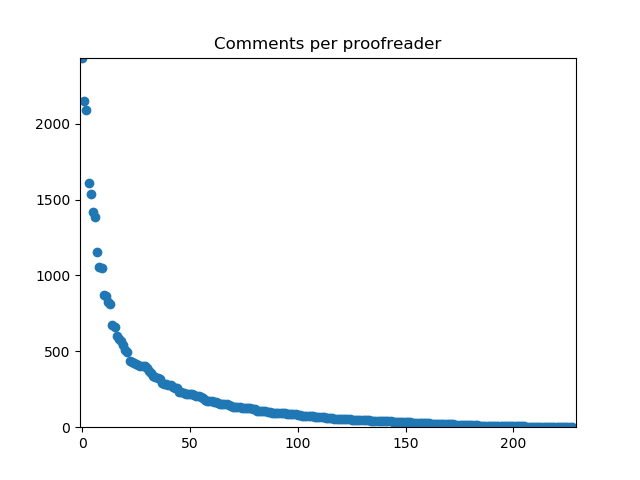
\includegraphics[height=.6\textheight]{commentsperproofreader_p.png}
228 different accounts have participated in commenting. 
}

\frame{
\frametitle{Proofreaders per book}
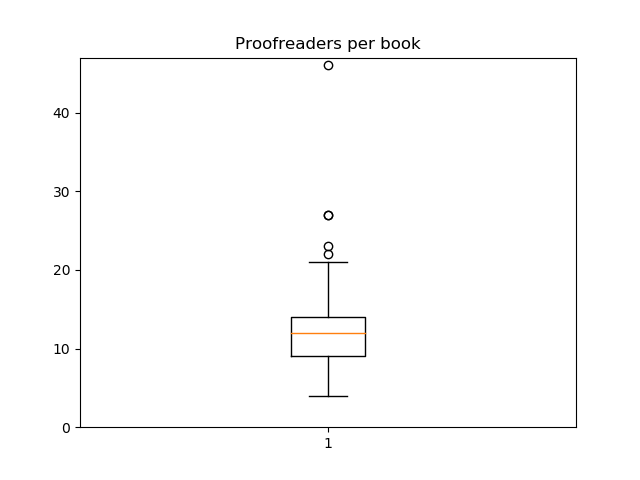
\includegraphics[height=\textheight]{proofreadersperbook.png}
  }

\frame{
\frametitle{Text analysis}
  
\includegraphics[width=\textwidth]{commenttitlebody.png}
  \begin{itemize}
    \item  
A PaperHive comment has a succinct title (<40 characters)
    \item 
optional body, with more  elaborate information 
  \end{itemize}
}

\frame{
\frametitle{Title length and body length}
  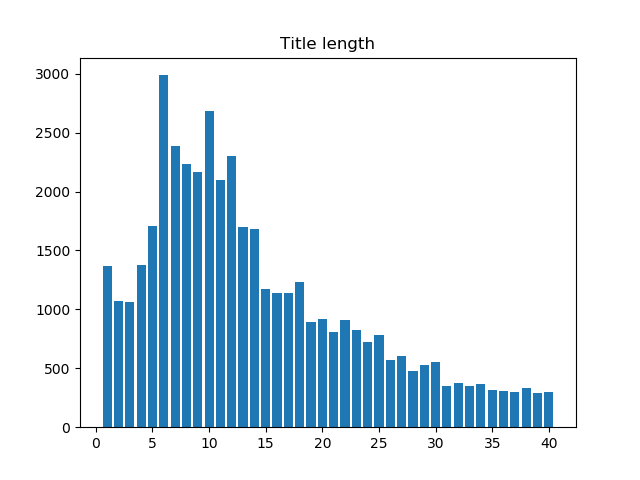
\includegraphics[height=.6\textheight]{titlelength_b.png}
  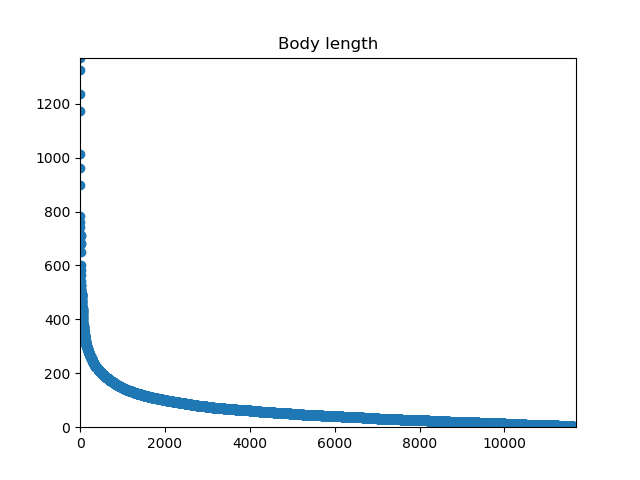
\includegraphics[height=.6\textheight]{bodylength_p.png}
}

\section{Creation of the corpus}
\frame{
\frametitle{Hypotheses about\\ proofreaders}
%   \includegraphics[height=.6\textheight]{./path/to/graphicsfile}
  \begin{enumerate}
    \item \textbf{Proofreaders fall into two types. Type 1 will focus on small details; type 2 will focus on the big picture. }
    \item \textbf{Proofreading comments will diminish as the proofreader moves along. Comments will become fewer due to fatigue, and average comment length will go down due to repetition of previous remarks as ``see above''.}
  \end{enumerate}
}
 
\frame{
\frametitle{Hypothesis 1:\\ proofreader types}
%   \includegraphics[height=.6\textheight]{./path/to/graphicsfile}
  \begin{itemize}
    \item  
Type 1: many comments but short (``comma missing'')
    \item 
    Type 2: few comments, but longer, in-depth
  \end{itemize}
} 

\frame{
\frametitle{Computation}
%   \includegraphics[height=.6\textheight]{./path/to/graphicsfile}
  \begin{itemize}
    \item For every book
    \begin{itemize}
      \item 
    rank all participating proofreaders by amount of comments 
    \item rank all participating proofreaders by average length of comments 
    \item plot the two against each other 
    \end{itemize}
  \end{itemize}
}

\frame{
\frametitle{Example of a plot\\ for Hypothesis 1}
  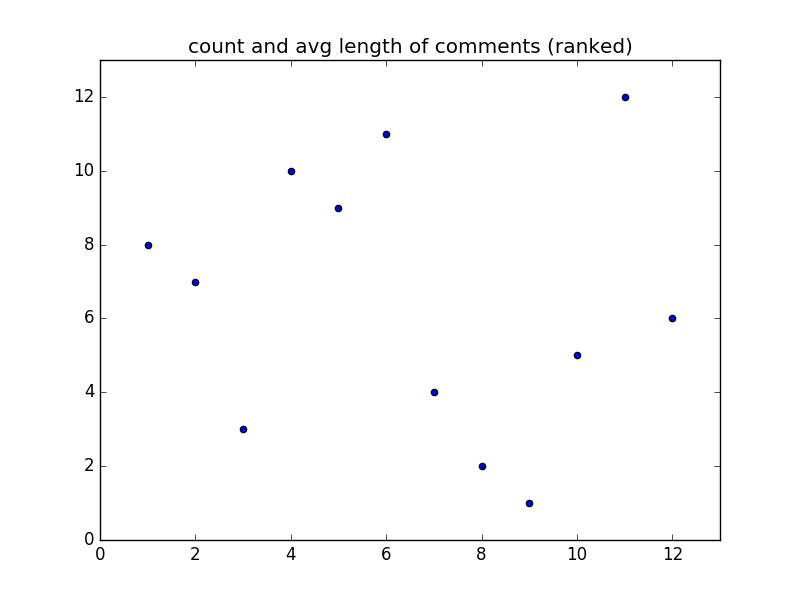
\includegraphics[height=.6\textheight]{allscatterx.png}
\begin{itemize}
  \item 12 proofreaders participated 
  \item their respective ranks are given by the dots. 
  \begin{itemize}
    \item e.g. \#3 in one rank is also \#3 in the other, but \#1 on one is \#8 in the other 
  \end{itemize}
  \item data from one book insufficient
\end{itemize}

  }

\frame{
\frametitle{Combination of all books}
  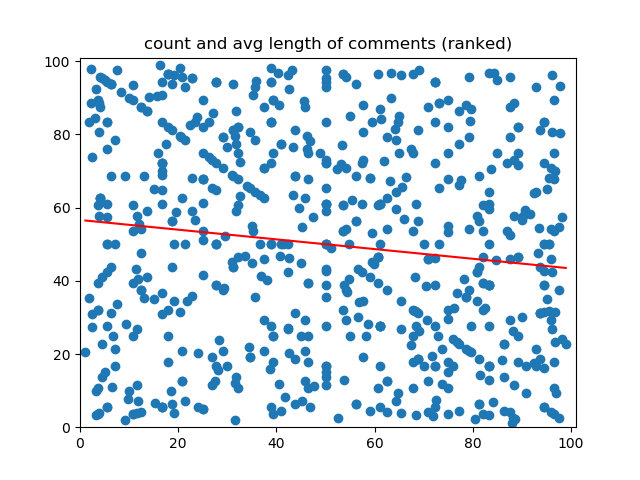
\includegraphics[height=.6\textheight]{allscatter.png}
  \begin{itemize}
    \item Ranks are normalized to centiles
    \item best fit given by red line
    \item indeed a weak negative correlation
  \end{itemize}
}
\frame{
\frametitle{Result hypothesis \#1}
%   \includegraphics[height=.6\textheight]{./path/to/graphicsfile}
  \begin{itemize}
    \item Hypothesis \#1 is confirmed
    \begin{itemize}
      \item 
proofreaders with more comments have shorter comments
      \item proofreaders with longer comments comment less 
    \end{itemize}
  \end{itemize}
}

\frame{
\frametitle{Hypothesis \#2: reviewer fatigue}
%   \includegraphics[height=.6\textheight]{./path/to/graphicsfile}
\textbf{Hypothesis 2 : Proofreading comments will diminish as the proofreader moves along. Comments will become fewer due to fatigue, and average comment length will go down due to repetition of previous remarks as ``see above''.}
}

\frame{
\frametitle{\mbox{Computation for Hypothesis \#2}}
%   \includegraphics[height=.6\textheight]{./path/to/graphicsfile}
  \begin{itemize}
    \item for every book 
     ~~for every proofreader 
       ~~~~for every comment
        \begin{itemize}
          \item compute relative length (e.g. 0.67 of the average)
          \item compute relative position (front, middle, back)
          \item store the tuple (relative position, relative length)
          \item A dot at (0.5, 5) means that there was a comment in the middle of the relevant stretch whose length was 5 times the average comment length. 
        \end{itemize}
\item the relative position can be pegged to the linear order of comments, or to the pages
    \end{itemize}
}

\frame{
\frametitle{Plot for Hypothesis \#2\\ based on linear order }
  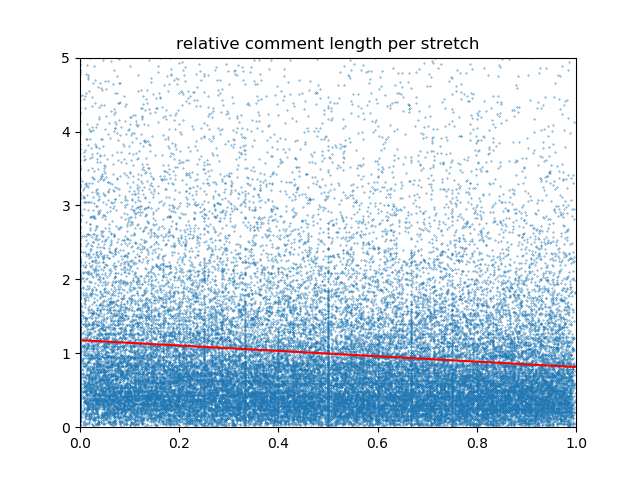
\includegraphics[height=\textheight]{stretches.png}
}

\frame{
\frametitle{Plot for Hypothesis \#2\\ based on page position }
  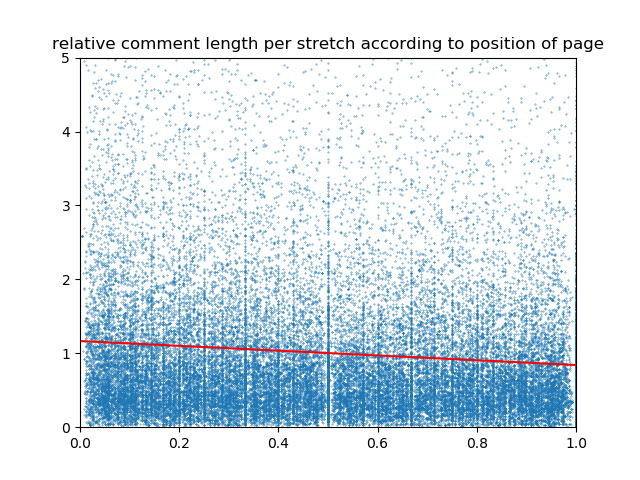
\includegraphics[height=\textheight]{stretchespages.png}
}

\frame{
\frametitle{Results for Hypothesis \#2\\ ``reviewer fatigue''}
%   \includegraphics[height=.6\textheight]{./path/to/graphicsfile}
  \begin{itemize}
    \item  Hypothesis is confirmed 
    \begin{itemize}
      \item the later in the document a comment is, the shorter it will be 
      \item the first comment will be about 110\% of the average, while the last one will be 90\% of the average.
      \item effect not very strong,  but discernible
    \end{itemize}
  \end{itemize}
}

\frame{
\frametitle{Discussion}
%   \includegraphics[height=.6\textheight]{./path/to/graphicsfile}
  \begin{itemize}
    \item  Main aim: methodological
    \item Proofreading comments are a by-product of open publishing 
    \begin{itemize}
      \item In traditional publishing models, these data would not be available
    \end{itemize}
    \item Once the documents, processes, and formats are opened up, novel research questions can emerge which would not have been possible under a closed setup.  
    \item Implications for psychology of reading for instance.
  \end{itemize}
}

\section{The ecosystem}
\frame{
\frametitle{Do researchers take on different roles? }
%   \includegraphics[height=.6\textheight]{./path/to/graphicsfile}
  \begin{itemize}
    \item  There are 908 people with the role ``author'' at LangSci Press 
    \item There are 228 proofreaders 
    \item 27 researchers have taken up both roles
    \begin{itemize}
      \item 16 started as authors, and became proofreaders later 
      \item 11 started as proofreaders, and became authors later
      \item Movement between the author pool and the proofreader pool in both directions. 
    \end{itemize}
  \end{itemize}
}

\frame{
\frametitle{Conclusions}
%   \includegraphics[height=.6\textheight]{./path/to/graphicsfile}
  \begin{itemize}
    \item  
    \item 
  \end{itemize}
}
\section{Conclusions}
\frame{
\frametitle{Conclusions}
%   \includegraphics[height=.6\textheight]{./path/to/graphicsfile}
  \begin{itemize}
    \item  
Community proofreading is a novel way of engaging the community
    \item 
only possible for Open Access publications 
\item 
workable implementation with 50+ books and 200+ researchers
\item 
can compare to traditional proofreading 
\item 
by-product data can be used for novel research questions
\begin{itemize}
  \item proofreader typology 
  \item proofreader fatigue
\end{itemize}
\item flow back and forth between the group of authors and the group of proofreaders
\item healthy ecosystem 
\item researchers from different backgrounds at different stages of their career contribute their respective expertises to creating and improving manuscripts.
  \end{itemize}
}
\frame{
\frametitle{Thank you}
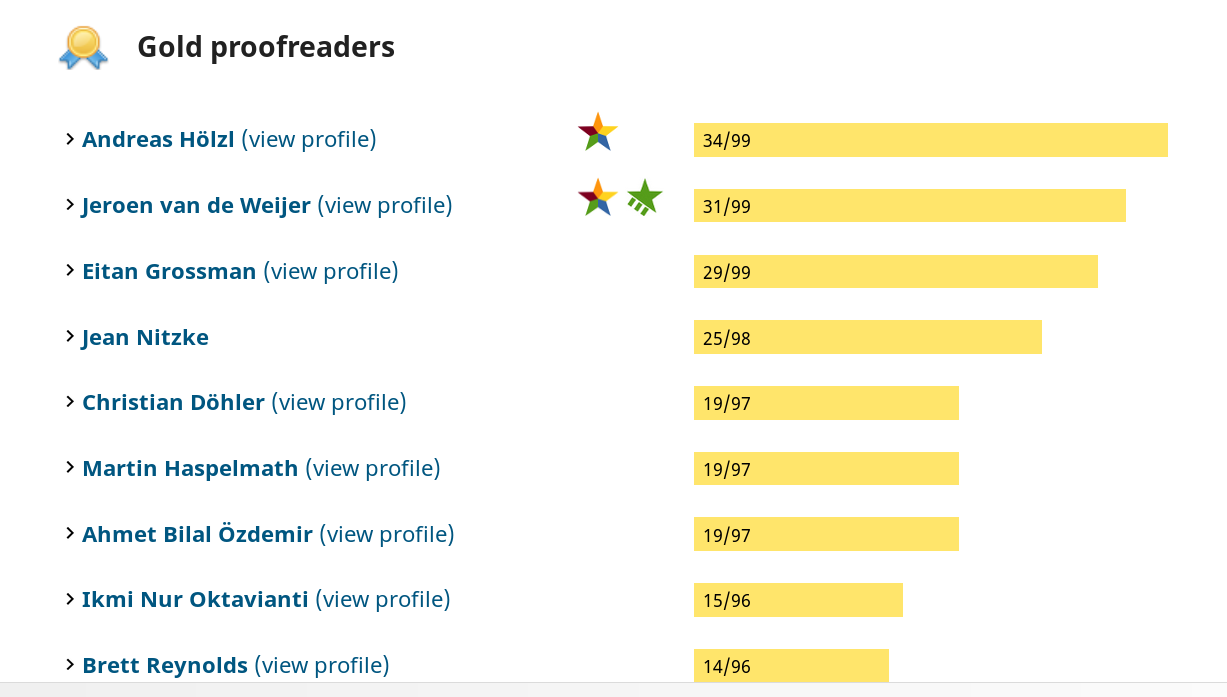
\includegraphics[height=.6\textheight]{halloffame.png}
}
\end{document}
